%Be more precise about what the system should and should not satisfy.
%Be sure to use the vocabulary introduced in the problem analysis.
\chapter{Requirements specification}

\subsection{The game play}%Cebrail
There are several things that a good game should include. The most important
and essential are:

\begin{enumerate}
\item Story
\item Great design
\item Easy to understand
\item Easy control
\item Sound effects
\end{enumerate}

Even though our project mainly focuses on implementing advanced algorithms, the gameplay
can not be ignored. Without a meaningful and understandable game, the advanced features will
be not as recognizable.

\subsection{The algorithms}
In order to implement the enemy motions and map generation, we'll have to create our
own algorithms.



\subsection{Timeplan} %Cebrail
Our timeplan follows an agile development system called waterfall.
The waterfall system is a sequential design process.
It is designed to get through the project phases and have a product as soon as
possible. The phases in our project can be seen in the figure below.

\subsubsection{Project management}
When the waterfall ends and we still have time
we will go back to the start and check for new requirements
and the whole waterfall process starts again.
The report is both written seamlessly and separately in the end of the project,
therefore it does not has to be illustrated, as it will create confusion.

\begin{figure}[h]
  \centering
  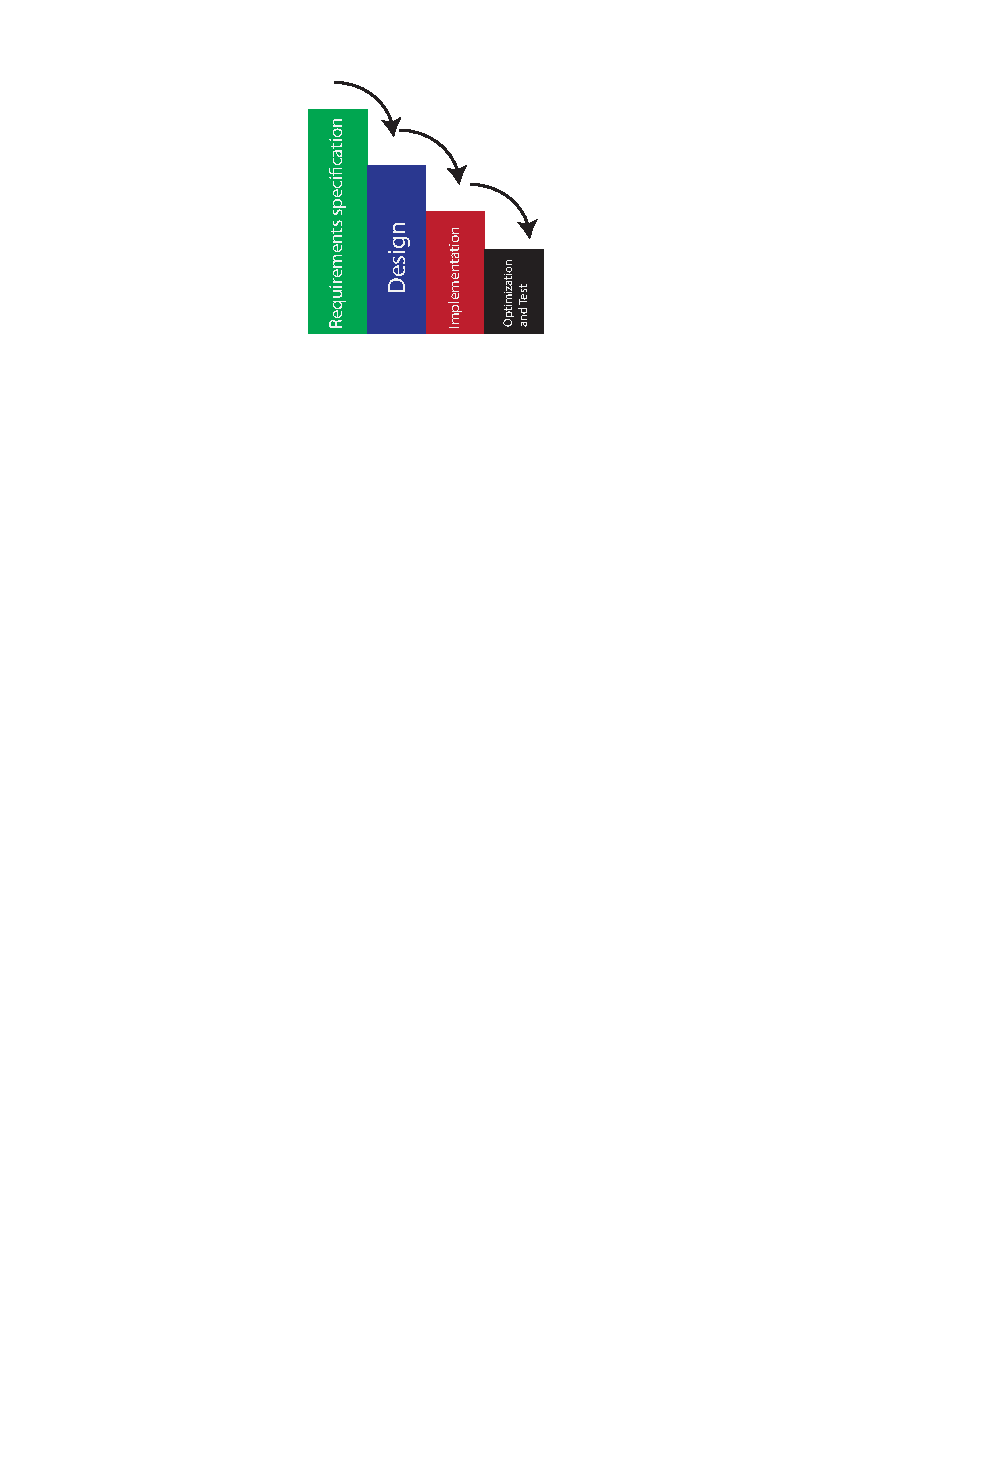
\includegraphics[scale=0.6]{Figures/Waterfall}
  \caption{An overview of the waterfall time plan.}
\label{fig:Waterfall}
\end{figure}


\subsubsection{Tasks management}%Cebrail
When providing the tasks we use the timeboxing method.
This method increases the productivity significantly.
Timeboxing works by breaking a big task into smaller tasks with better manageable time frames.
It kinda works like a stopwatch. The following table shows the timeboxes we have
created during the project.

% Please add the following required packages to your document preamble:
% \usepackage[table,xcdraw]{xcolor}
% If you use beamer only pass "xcolor=table" option, i.e. \documentclass[xcolor=table]{beamer}

\begin{table}[h]
\begin{tabular}{llll}
\rowcolor[HTML]{BBDAFF} 
{\color[HTML]{000000} \textbf{8-10}} & {\color[HTML]{000000} \textbf{11-13}} & {\color[HTML]{000000} \textbf{14-15}} & {\color[HTML]{000000} \textbf{16-17}} \\
Code exercise                        & Enemies                               & Scene generation (simple)             & Graphics                              \\
Game design                          & Collision Detection                   & Player                                & Sprites                               \\
Class Design                         & AI                                    &                                       & Map generation                        \\
                                     & Input                                 &                                       &                                       \\
Report                               & Report                                & Report                                & Report                                \\
                                     &                                       &                                       &                                       \\
\rowcolor[HTML]{BBDAFF} 
\textbf{18-90}                       & \textbf{19}                           & \textbf{20}                           & \textbf{22-25}                        \\
Endgame                              & Scene generation                      & Sprites                               & Optimization                          \\
Map generation                       & Optimization                          & Sound                                 &                                       \\
                                     & Attack                                & Optimization                          &                                       \\
                                     &                                       & Animation                             &                                       \\
Report                               & Report                                & Report                                &                                      
\end{tabular}
\caption{The timeboxes are seperated per week}
\end{table}
